% Euclidean Handout Number seven
\documentclass{tufte-handout}

%\geometry{showframe}% for debugging purposes -- displays the margins

%%%% Packages to make things pretty
\usepackage{amsmath,amsthm}
\usepackage{booktabs}
\usepackage{graphicx}
\setkeys{Gin}{width=\linewidth,totalheight=\textheight,keepaspectratio}
\graphicspath{{graphics/}}
\usepackage{units}
\usepackage{fancyvrb}
\fvset{fontsize=\normalsize}
\usepackage{multicol}
\usepackage{pdfpages}

%%%% Theorem Environments
\theoremstyle{definition}
\swapnumbers
\newtheorem{problem}{Problem}[section]
\newtheorem{conjecture}[problem]{Conjecture}
\newtheorem*{definition}{Definition}
\newtheorem*{theorem}{Theorem}
\newtheorem{question}[problem]{Question}
\newtheorem{challenge}[problem]{Challenge}
\newtheorem*{postulate}{Postulate}

%%%%%

\title{Euclidean Geometry:\\An Introduction to Mathematical Work}
\author[]{Math 3600}
\date{Fall 2018}

\begin{document}

\maketitle

\begin{marginfigure}
    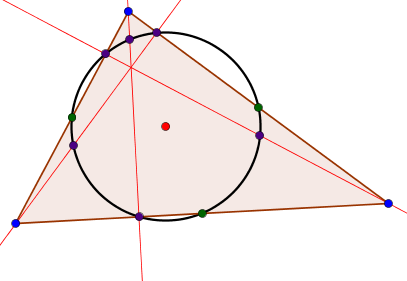
\includegraphics{NPC}
\end{marginfigure}

\setcounter{section}{7}

\section{Deeper Into Triangles}

So far, our most useful tools have been facts about triangles. Euclid makes a pretty thorough study of triangles, but he doesn't cover everything he could. 
Here we shall plug  gaps in Book I with some very useful understanding.

\begin{problem}
\label{prob:triangle-inequality}
Show how to construct three segments which are not congruent to the sides of any triangle.
\end{problem}


\begin{definition}
\label{defn:right-triangles}
A triangle is said to be \emph{right} if one of its angles is a right angle. 
The side opposite the right angle is called the \emph{hypotenuse}. 
The other sides are called \emph{legs}.
\end{definition}

\begin{conjecture}
\label{conj:RASS}
Let $ABC$ and $DEF$ be two right triangles, with the angles at $A$ and $D$ right angles. 
Suppose that $BC$ is congruent to $EF$ and $AB$ is congruent to $DE$. 
Then the triangles are congruent.
\marginnote{This is sometimes called the \emph{hypotenuse-leg} theorem.}
\end{conjecture}

\begin{conjecture}
\label{conj:ASS}
If we weaken the hypothesis of the previous conjecture so that the angles $A$ and $D$ are still congruent but no longer assumed to be right angles, and leave the other hypotheses intact, the conclusion still holds.
\end{conjecture}

Right triangles are very useful objects. 
But we need to know when we have a right angle! 
Here is a wonderful characterization of right angles.

\begin{conjecture}
\label{conj:thales1}
If $AB$ is the diameter of a circle and $C$ lies on the circle, then angle $\angle ACB$ is a right angle.
\end{conjecture}

\begin{conjecture}
\label{conj:thales2}
If $\angle ACB$ is a right angle, then $C$ lies on the circle with diameter $AB$.
\end{conjecture}

Note that, together, Conjectures \ref{conj:thales1} and \ref{conj:thales2} yield this result:
\begin{theorem}[Thales' Theorem] 
Let $A, B, C$ be three points. 
The angle $\angle ACB$ is a right angle if and only if $C$ lies on the circle with diameter $AB$.
\end{theorem}

\marginnote[-160pt]{It is mathematical folklore that Thales' theorem is the oldest theorem. 
That is, this theorem was the first one that was given what would today be called a proof. 
Thales is thought to be the originator of our axiomatic method of working from assumed statements (axioms or postulates) to prove true statements (theorems) which followed only from logical reasoning. 
It is also part of the folklore that Thales was so overjoyed at the discovery of this theorem and proof that he sacrificed an ox as thanksgiving. 
I don't know if this is true--I've also heard such a story associated with the Pythagoreans and their famous triangle theorem, though it was 100 oxen. 
Euclid's \emph{Elements} is really an ancient Greek textbook. 
It seems clear that the method of axiomatic work typical of mathematics originated somehow with the Greeks before Euclid--say with Thales or with the Pythagoreans. But all of the literature has been lost to the ages.}

This is a case of a set of \emph{equivalent conditions}. We have stated it
here with ``if and only if'' language, but we also could have said ``for angle $\angle ACB$ to be a right angle it is necessary and sufficient that $C$ lies on the circle with diameter $AB$.'' The necessity is in Conjecture \ref{conj:thales2}. The sufficiency is in Conjecture \ref{conj:thales1}.
%Whatever choice of terms we use, we are saying that knowing one thing (that $\angle ACB$ is a right angle) is exactly the same situation as knowing another thing (that $C$ lies on the circle with diameter $AB$.)

\vfill
\end{document}
